\documentclass{classrep}
\usepackage[utf8]{inputenc}
\usepackage{color}
\usepackage{listings}
\usepackage{graphicx}

\graphicspath{ {../uml/} }

\studycycle{Informatyka, studia STACJONARNE, I st.}
\coursesemester{VI}

\coursename{Komputerowe systemy rozpoznawania}
\courseyear{2020/2021}

\courseteacher{dr inż. Marcin Kacprowicz}
\coursegroup{poniedziałek, 12:00}

\author{
  \studentinfo{Maciej Lewandowski}{224357} \and
  \studentinfo{Kamil Dike}{224282} }

\title{Projekt 1. Klasyfikacja dokumentów tekstowych}

\begin{document}
\maketitle

Opis projektu ma formę artykułu naukowego lub raportu z zadania
badawczego/doświadczalnego/obliczeniowego (wg indywidualnych potrzeb związanych np. z
pracą inżynierską/naukową/zawodową). \\
\indent {\bf Wybrane sekcje (rozdziały sprawozdania) są uzupełniane wg wymagań w
opisie Projektu 1. i Harmonogramie ZAJĘĆ na WIKAMP KSR jako efekty zadań w~poszczególnych tygodniach}. 

\section{Cel projektu}
Celem zadania jest stworzenie systemu klasyfikującego teksty w zależności od kraju który jest opisywany przez tekst.
\indent System został oparty o metodę k-NN. Ponad to została przeanalizowana skuteczność działania programu w odniesieniu do nietraktowanego wektora cech.

\section{Klasyfikacja nadzorowana metodą $k$-NN}
Metoda $k$-NN służy do klasyfikacji obiektów. Opiera się na założeniu podobieństwa obiektów blisko położonych w przestrzeni cech. Jak podaje  założenia dla algorytmu:
\newline $numclass$ - liczba rozpoznawanych klas
\newline $dim$ - wymiar przestrzeni cech
\newline $num$ - liczba obiektów ciągu uczącego
\newline $sampl[1... num][1...dim+1]$ - ciąg uczący
\newline $rec$ - identyfikator rozpoznanego obiektu
\newline $obj[1...dim]$ - rozpoznawany obiekt
\newline $dist(sampl[k],obj)$ - funkcja podająca odległość między i-tym elementem ciągu uczącego a rozpoznawanym obiektem  
\newline $k$ - zmienna określająca ilość uwzględnianych sąsiadów
\newline $tab[1...num][1...2]$ - tablica odległości
\newline $sort(tab)$ - funkcja sortująca tablicę
\newline $fun[1..numclass]$ - tabela wartości funkcji przynależności
\newline $pointmax(fun)$  - funkcja wskazująca numer klasy, dla której wartość przynależności jest maksymalna. Algorytm według składa się z następujących kroków:
\newline
\begin{verbatim}
 1.  wyzeruj tablicę fun
 2.  wykonaj pętlę s od i=1 do num
 3.  w pętli s przyporządkuj elementowi tablicy tab[i][1]
     wynik wywołania funkcji dist(sampl[i],obj)
 4.  w pętli s przyporządkuj elementowi tablicy tab[i][2]
     element tablicy sampl[i][dim+1]
 5.  zakończ pętlę s
 6.  wykonaj sortowanie tablicy sort(tab)
 7.  rozpocznij pętlę q od i=1 do i=k
 8.  w pętli q przyporządkuj elementowi tablicy fun[tab[i][2]]
     element tablicy fun[tab[i][2]]+1
 9.  zakończ pętlę q
 10. przyporządkuj zmiennej rec wynik funkcji pointmax(fun)
\end{verbatim}

%\begin{enumerate}
%\item wyzeruj tablicę $fun$
%\item wykonaj pętlę $s$ od $i=1$ do $num$
%\item w pętli $s$ przyporządkuj elementowi tablicy $tab[i][1]$ wynik wywołania funkcji $dist(sampl[i],obj)$
%\item w pętli $s$ przyporządkuj elementowi tablicy $tab[i][2]$ element tablicy $sampl[i][dim+1]$
%\item zakończ pętlę $s$
%\item wykonaj sortowanie tablicy $sort(tab)$
%\item rozpocznij pętlę $q$ od $i=1$ do $i=k$
%\item w pętli $q$ przyporządkuj elementowi tablicy $fun[tab[i][2]]$ element tablicy $fun[tab[i][2]]+1$
%\item zakończ pętlę $q$
%\item przyporządkuj zmiennej $rec$ wynik funkcji $pointmax(fun)$
%\end{enumerate}
\indent Algorytm jako dane wejściowe pobiera obiekt do klasyfikacji $obj$ oraz zmienną przechowującą informacje o klasie do którego zostanie przyporządkowany $rec$.Odległość dwóch obiektów określana jest poprzez określoną metrykę. Porównywane będą wektory cech reprezentujące obiekty.


\subsection{Ekstrakcja cech, wektory cech}
Na potrzeby reprezentacji obiektów poprzez wektory cech wybrano cechy:
\begin{enumerate}

\item Liczba słów w dokumencie
\begin{equation}
v_{1}=\hat{A}\label{eq:eps}
\end{equation}
,gdzie 
\newline $A$ oznacza artykuł taki, że $A=[s_1,s_2,s_3,. . . ,s_T]$
\newline $s_i$ oznacza $i$- te słowo w artykule
\newline $\hat{A}$ oznacza moc zbioru $A$

\item Wartość logiczna z logiki trój-wartościowej określająca dominujący rodzaj jednostek występujących w tekście. Wartość cechy 1 oznacza że dominują w artykule jednostki układu SI. Wartość cechy 0 oznacza że w artykule dominują jednostki układu Imperialnego. Wartość cechy 1/2 oznacza że w artykule nie dominują jednostki układu SI anie jednostki układu imperialnego.
\begin{equation}
v_{2}=l(A) \label{eq:eps}
\end{equation}
,gdzie
\newline $l:\mathcal{A} \rightarrow \{0,\frac{1}{2},1\}$, $l$ funkcja przyporządkowywuje artykułowi wartość logiczną 0, 1/2 albo 1 w zależności od ilości wystąpień jednostek danego typu(si/imperialne).
\newline $\mathcal{A}$ oznacza zbiór wszystkich możliwych wektorów reprezentujących artykuły.

\item Najczęściej występujący miesiąc
\begin{equation}
v_{3}=m(A) \label{eq:eps}
\end{equation}
,gdzie
\newline $m:\mathcal{A} \rightarrow \{0,1,2,. . . ,12\}$, $m$ funkcja przyporządkowywująca artykułowi wartość całkowitą od 0 do 12, w zależności od ilości wystąpień danego miesiąca w zbiorze $A$.


\item Najczęściej występujący typ spółki/firmy
\begin{equation}
v_{4}=f(max(k(A,G_S))) \label{eq:eps}
\end{equation}
,gdzie
\newline $\mathcal{G}$ zbiór wszystkich możliwych wektorów słów kluczowych
\newline $G_S = [x_1,x_2,x_3,. . . , x_j]$ wektor słów kluczowych rodzajów spółek
\newline $x_i$ oznacza $i$-te słowo kluczowe
\newline $\mathcal{H}$ zbiór wszystkich możliwych wektorów częstości występowania słów kluczowych
\newline $H$ wektor częstości występowania słów kluczowych
\newline $f:\mathcal{H} \rightarrow \mathcal{G}$, f jest funkcją przyporządkowującą zbiór częstości do zbioru słów kluczowych
\newline $k:\mathcal{A},\mathcal{G}\rightarrow\mathcal{H}$, k jest funkcją zwracającą wektor częstości dla zapewnionego artykułu oraz wektora słów kluczowych

\item Najczęściej występująca w tekście nazwa giełdy
\begin{equation}
v_{5}=f(max(k(A,G_G))) \label{eq:eps}
\end{equation}
,gdzie
\newline $G_g = [x_1,x_2,x_3,. . . , x_j]$ wektor słów kluczowych nazw giełd

\item Najczęściej występująca nazwa morza lub oceanu
\begin{equation}
v_{6}={f(max(k(A,G_M)))}\label{eq:eps}
\end{equation}
,gdzie
\newline $G_M = [x_1,x_2,x_3,. . . , x_j]$ wektor słów kluczowych nazw mórz i oceanów


\item Względna ilość słów o długości do 4 znaków
\begin{equation}
v_{7}=\frac{c(A,0,4)}{v_1}\label{eq:eps}
\end{equation}
,gdzie
\newline $c:\mathcal{A},N,M\rightarrow P$ c jest funkcją zliczającą ilość słów o długości od n do m znaków
\newline $N = \{n:n\in\mathrm{N} \land n>0\}$
\newline $M = \{m:m\in\mathrm{N} \land m>n\}$
\newline $P = \{p:p\in\mathrm{N}\}$

\item Względna ilość słów o długości od 4 do 8 znaków
\begin{equation}
v_{8}=\frac{c(A,4,8)}{v_1}\label{eq:eps}
\end{equation}


\item Względna ilość słów o długości od 8 znaków
\begin{equation}
v_{9}=\frac{c(A,8,\infty)}{v_1}\label{eq:eps}
\end{equation}

\item Najczęściej występujący rok w artykule
\begin{equation}
v_{10}=yr(A)\label{eq:eps}
\end{equation}
,gdzie
\newline $yr:\mathcal{A}\rightarrow\mathcal{P}$, $yr$ to funkcja zwracająca najczęściej występującą datę w tekście


\item Ilość cen w tekście
\begin{equation}
v_{11}=dl(A)\label{eq:eps}
\end{equation}
,gdzie
\newline $dl:\mathcal{A}\rightarrow\mathcal{P}$, $yr$ to funkcja zwracająca najczęściej występujący rok w tekście


\item Liczba unikalnych słów
\begin{equation}
v_{12}=us(A)\label{eq:eps}
\end{equation}
,gdzie
\newline $us:\mathcal{A}\rightarrow\mathcal{P}$, $yr$ to funkcja zwracająca ilość różnych słów w tekście
\end{enumerate}

\subsection{Miary jakości klasyfikacji}
Celem miar jakości klasyfikacji jest zbadanie dokonanej klasyfikacji. Ze względu na brak miary idealnej posłużymy się paroma następującymi miarami:
\begin{enumerate}
\item{accuracy}
\item{precision}
\item{recall}
\item{F1}
\end{enumerate}
Do wyznaczenia miar jakości klasyfikacji korzystamy z tablicy pomyłek. Spis oznaczeń:
\newline $TP$ - prawdziwie pozytywna klasyfikacja
\newline $FP$ - fałszywie pozytywna klasyfikacja
\newline $FN$ - fałszywie negatywna klasyfikacja
\newline $TN$ - prawdziwie negatywna klasyfikacja
\newline
\begin{enumerate}
\item[TP]{\textit{Przykład dla $TP$} Jeśli obiekt $A$ w rzeczywistości należy do klasy $\mathcal{A}$, i zostanie sklasyfikowany do klasy $\mathcal{A}$ wówczas klasyfikacja jest uznawana za prawdziwie pozytywną $TP$.}
\item[FP]{\textit{Przykład dla $FP$} Jeśli obiekt $A$ w rzeczywistości nie należy do klasy $\mathcal{A}$, i zostanie sklasyfikowany do klasy $\mathcal{A}$ wówczas klasyfikacja jest uznawana za fałszywie pozytywną $FP$.}
\item[FN]{\textit{Przykład dla $FN$} Jeśli obiekt $A$ w rzeczywistości należy do klasy $\mathcal{A}$, i nie zostanie sklasyfikowany do klasy $\mathcal{A}$ wówczas klasyfikacja jest uznawana za fałszywie negatywną $FN$.}
\item[TN]{\textit{Przykład dla $TN$} Jeśli obiekt $A$ w rzeczywistości nie należy do klasy $\mathcal{A}$, i nie zostanie sklasyfikowany do klasy $\mathcal{A}$ wówczas klasyfikacja jest uznawana za prawdziwie negatywną $TN$.}
\end{enumerate}


\subsubsection{Accuracy}
Dokładność wyraża się wzorem:
\begin{equation}
ACC=\frac{\Sigma TP}{\Sigma populacja} \label{eq:eps}
\end{equation}
\subsubsection{Precision}
Precyzja wyraża się wzorem:
\begin{equation}
PPV=\frac{\Sigma TP}{\Sigma TP + \Sigma FP} \label{eq:eps}
\end{equation}
\subsubsection{Recall}
Czułość wyraża się wzorem:
\begin{equation}
TPR=\frac{\Sigma TP}{\Sigma TP + \Sigma FN} \label{eq:eps}
\end{equation}
\subsubsection{F1}
Miarę F1 wyraża się wzorem:
\begin{equation}
TPR=2*\frac{PPV*TPR}{PPV + TPR} \label{eq:eps}
\end{equation}


\section{Klasyfikacja z użyciem metryk i miar podobieństwa tekstów}
Program umożliwia wybór trzech metryk do porównywania wektorów cech: metryki miejskiej, amplitudy kosinusowej oraz odległości euklidesowej.
\begin{enumerate}
\item[Metryka miejska]{\begin{equation}
\rho_{C}(X,Y) = {{\Sigma}^{n}}_{i=1} |x_i-y_i|\label{eq:eps}
\end{equation}}
\item[Amplituda kosinusowa]{\begin{equation}
r_{ca}(V_1,V_2) = \frac{|{{\Sigma}^{n}}_{i=1} v_{1i}\cdot v_{2i}|}{\sqrt{{{\Sigma}^{n}}_{i=1} v_{1i}^2 \cdot {{\Sigma}^{n}}_{i=1} v_{2i}^2}}\label{eq:eps}
\end{equation}}
\item[Odległość euklidesowa]{\begin{equation}
\rho_{E}(X,Y) = \sqrt{{{\Sigma}^{n}}_{i=1} (x_i-y_i)^2}\label{eq:eps}
\end{equation}}
\end{enumerate}

Jako metrykę tekstową do ekstrakcji cech tekstowych zastosowano metodę \textit{trigramów}, opisaną poniższym równaniem.
\begin{equation}
sim_{3}(s_1,s_2) = \frac{1}{N-2} {{\Sigma}^{N-2}}_{i=1} h(i)\label{eq:eps}
\end{equation}
\newline , gdzie
\newline $N-2$ - ilość możliwych trój-elementowych podciągów.
\newline $h(i) = 1$ - jeśli trój-elementowy podciąg zaczynający się od $i$-tej pozycji w $s_1$ występuje przynajmniej raz w $s_2$, w innym przypadki $h(i)=0$.

\subsubsection{Wstępne wyniki miary accuracy}
Uruchomiono program w czterech konfiguracjach:
\newline Dla zbioru uczącego stanowiącego $60 proc$ oraz dla $17$ sąsiadów $ACC=0.7666$.
\newline Dla zbioru uczącego stanowiącego $60 proc$ oraz dla $3$ sąsiadów $ACC=0.7693$.
\newline Dla zbioru uczącego stanowiącego $30 proc$ oraz dla $17$ sąsiadów $ACC=0.7913$.
\newline Dla zbioru uczącego stanowiącego $30 proc$ oraz dla $3$ sąsiadów $ACC=0.7379$.



\section{Budowa aplikacji}
\subsection{Diagramy UML}

\subsubsection{Struktura aplikacji}
Aplikacja złożona jest z komponentów: extractor, features, knn, main, model, parser, utils. Struktura aplikacji została przedstawiona na rysunku \ref{app} na stronie \pageref{app}.

\begin{figure}
\label{app}
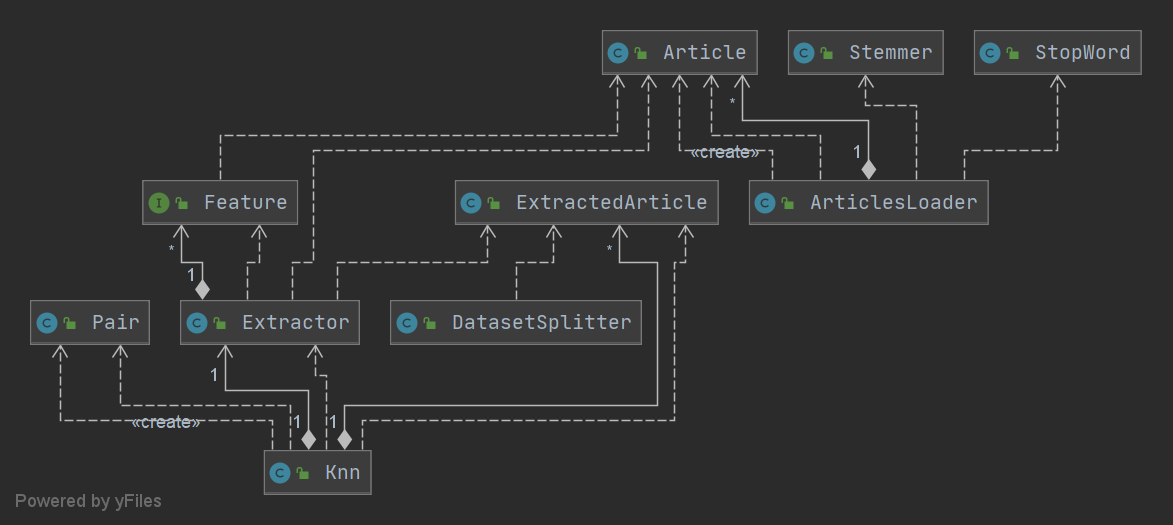
\includegraphics[scale=0.35]{App structure}
\caption{Struktura aplikacji}
\end{figure}


\subsubsection{extractor}
Pakiet ekstraktor udostępnia narzędzia umożliwiające ekstrakcję cech z tekstów. Pakiet ekstraktor zaprezentowano na rysunku \ref{extr} na stronie \pageref{extr}.
\begin{figure}
\label{extr}
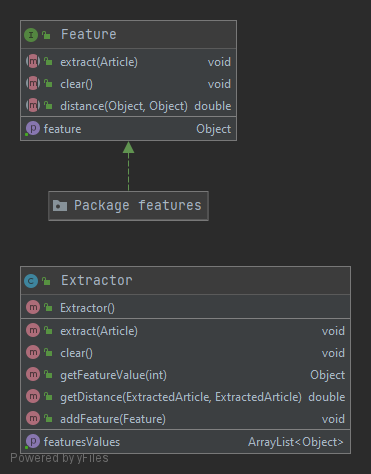
\includegraphics[scale=0.5]{Package extractor}
\caption{Pakiet extrator}
\end{figure}


\subsubsection{features}
Pakiet features udostępnia abstrakcję cechy oraz modeluje logikę konkretnych cech. Pakiet features zaprezentowano na rysunku \ref{feat} oraz \ref{feat2} na stronie \pageref{feat}.
\begin{figure}
\label{feat}
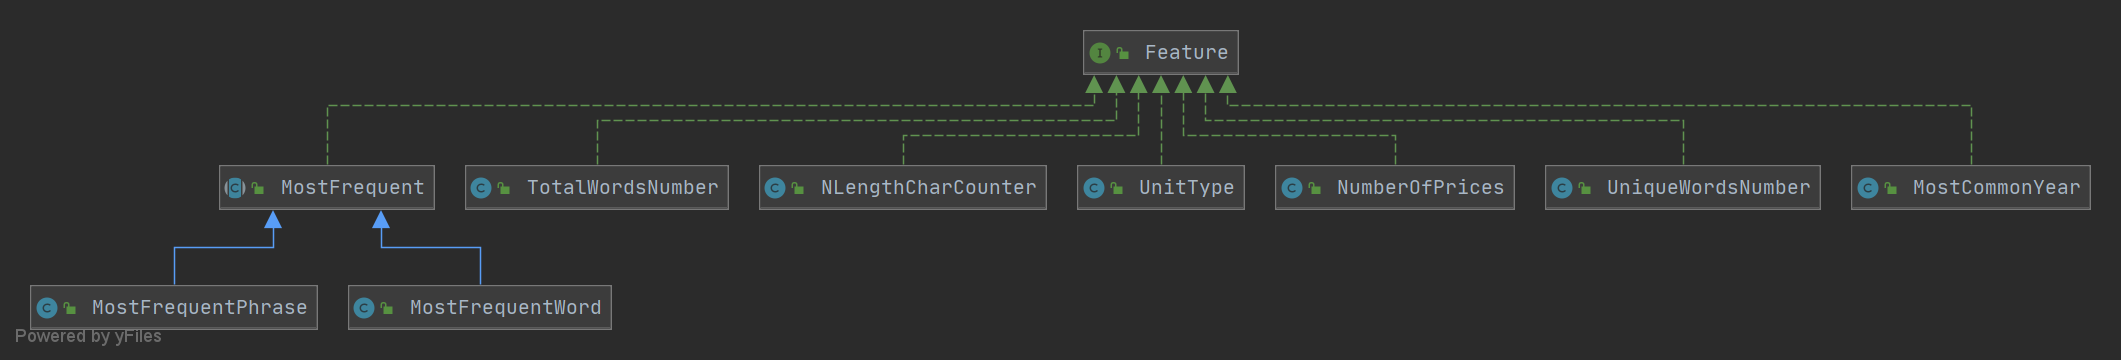
\includegraphics[scale=0.20]{Features structure}
\caption{Struktura pakietu features}
\end{figure}
\newline

\begin{figure}
\label{feat2}
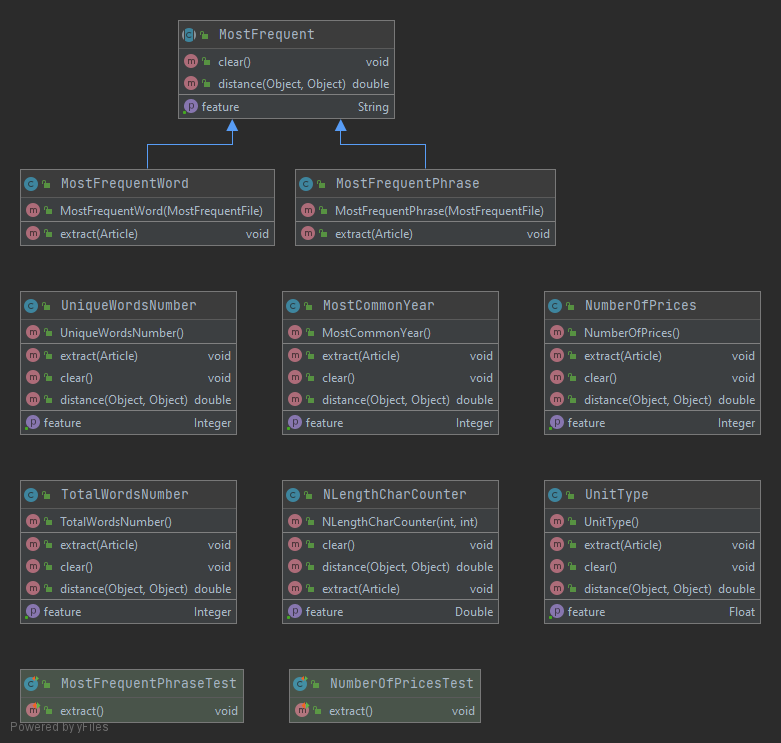
\includegraphics[scale=0.5]{Package features}
\caption{Pakiet features}
\end{figure}


\subsubsection{knn}
Pakiet knn udostępnia algorytm $k-NN$. Pakiet knn zaprezentowano na rysunku \ref{knn} na stronie \pageref{knn}.
\begin{figure}
\label{knn}
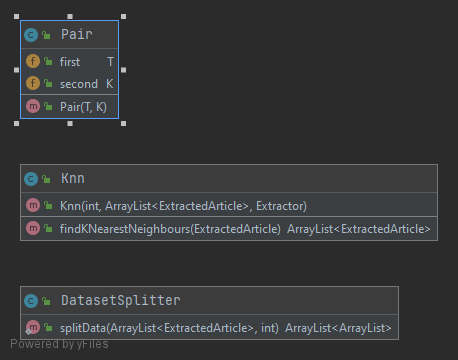
\includegraphics[scale=0.5]{Package knn}
\caption{Pakiet knn}
\end{figure}

\subsubsection{main}
Pakiet main stanowi wejście, oraz implementuje logikę CLI. Pakiet main zaprezentowano na rysunku \ref{main} na stronie \pageref{main}.

\begin{figure}
\label{main}
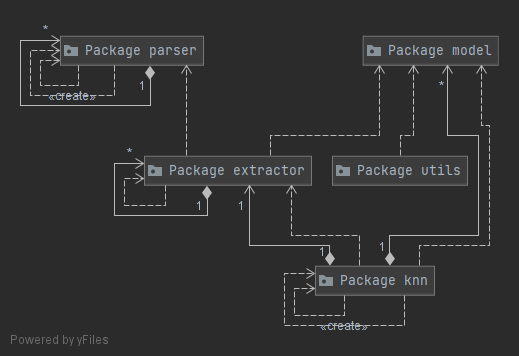
\includegraphics[scale=0.5]{Package main}
\caption{Pakiet main}
\end{figure}


\subsubsection{model}
Pakiet model dostarcza model danych dla artykułu reprezentowanego jako wektor cech oraz pozostałe wymagane modele danych. Pakiet model zaprezentowano na rysunku \ref{mdl} na stronie \pageref{mdl}.

\begin{figure}
\label{mdl}
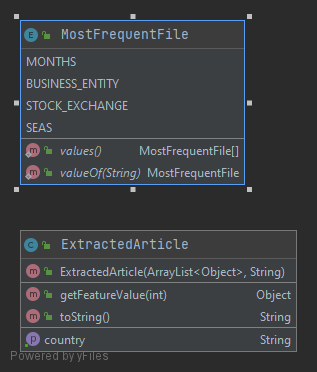
\includegraphics[scale=0.5]{Package model}
\caption{Pakiet model}
\end{figure}

\subsubsection{parser}
Pakiet parser udostępnia metody odpowiedzialne za przygotowanie tekstu przed ekstrakcją cech. Pakiet parser zaprezentowano na rysunku \ref{prs} na stronie \pageref{prs}.

\begin{figure}
\label{prs}
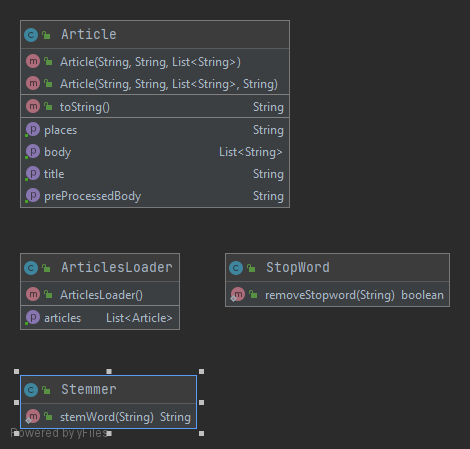
\includegraphics[scale=0.5]{Package parser}
\caption{Pakiet parser}
\end{figure}


\subsubsection{utils}
Pakiet utils udostępnia narzędziowe metody wykorzystywane przez pozostałe pakiety.  Pakiet utils zaprezentowano na rysunku \ref{utls} na stronie \pageref{utls}.
\begin{figure}
\label{utls}
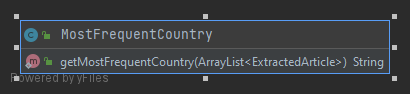
\includegraphics[scale=0.5]{Package utils}
\caption{Pakiet utils}
\end{figure}

\subsection{Prezentacja wyników, interfejs użytkownika} 
\subsubsection{Interfejs użytkownika}
Interfejs użytkownika jest w formie tekstowej. Poniżej pokazano przykładowe uruchomienie programu przy udziale zbioru treningowego $60 proc$, siedmiu sąsiadów, do klasyfikacji wykorzystano wszystkie kraje, oraz użyto wszystkich cech opisanych wyżej.
\begin{verbatim}
Okresl procent zbioru treningowego:
60
Okresl ilosc sasiadow KNN:
17
Wybierz interesujące kraje: 
0. Wszystkie
1. USA
2. UK
3. Japan
4. Canada
5. West-Germany
6. France
Y. Przejdz dalej
0
Wybierz interesujące metryki: 
0. Wszystkie
1. TotalWordsNumber
2. unitType
3. shortWords
4. middleWords
5. longWords
6. mostCommonYear
7. mostFrequentWordMonth
8. mostFrequentWordBusinessEntity
9. mostFrequentStockExchange
10. mostFrequentSea
11. numberOfPrices
12. uniqueWordsNumber
Y. Przejdz dalej
0
loading...
\end{verbatim}

Wynik wygenerowany przez program będzie następujący:

\begin{verbatim}
Dla usa _________
Dokladnosc: 0.766563241467421
Precyzja: 0.789354044326577
Czulosc: 0.9643601018282805
F1: 0.8681249999999999


Dla uk _________
Dokladnosc: 0.766563241467421
Precyzja: 0.165
Czulosc: 0.0889487870619946
F1: 0.11558669001751312


Dla japan _________
Dokladnosc: 0.766563241467421
Precyzja: 0.5
Czulosc: 0.0
F1: 0.0


Dla canada _________
Dokladnosc: 0.766563241467421
Precyzja: 0.5
Czulosc: 0.0
F1: 0.0


Dla west-germany _________
Dokladnosc: 0.766563241467421
Precyzja: 0.5
Czulosc: 0.0
F1: 0.0


Dla france _________
Dokladnosc: 0.766563241467421
Precyzja: 0.5
Czulosc: 0.0
F1: 0.0

\end{verbatim}


\section{Wyniki klasyfikacji dla różnych parametrów wejściowych}
Wyniki kolejnych eksperymentów wg punktów 2.-8. opisu projektu 1.  Wykresy i tabele
obowiązkowe, dokładnie opisane w ,,captions'' (tytułach), konieczny opis osi i
jednostek wykresów oraz kolumn i wierszy tabel.\\ 

{**Ewentualne wyniki realizacji punktu 9. opisu Projektu 1., czyli,,na ocenę 5.0'' i ich porównanie do wyników z
części obowiązkowej**.}\\

\noindent {\bf Sekcja uzupełniona jako efekt zadania Tydzień 05 wg Harmonogramu Zajęć
na WIKAMP KSR.}


\section{Dyskusja, wnioski}

Dokładne interpretacje uzyskanych wyników w zależności od parametrów klasyfikacji
opisanych w punktach 3.-8 opisu Projektu 1. 
Szczególnie istotne są wnioski o charakterze uniwersalnym, istotne dla podobnych zadań. 
Omówić i wyjaśnić napotkane problemy (jeśli były). Każdy wniosek/problem powinien mieć poparcie
w przeprowadzonych eksperymentach (odwołania do konkretnych wyników: wykresów,
tabel). \\
\underline{Dla końcowej oceny jest to najważniejsza sekcja} sprawozdania, gdyż prezentuje poziom
zrozumienia rozwiązywanego problemu.\\

** Możliwości kontynuacji prac w obszarze systemów rozpoznawania, zwłaszcza w kontekście pracy inżynierskiej,
magisterskiej, naukowej, itp. **\\

\noindent {\bf Sekcja uzupełniona jako efekt zadania Tydzień 06 wg Harmonogramu Zajęć
na WIKAMP KSR.}


\section{Braki w realizacji projektu 1.}
Wymienić wg opisu Projektu 1. wszystkie niezrealizowane obowiązkowe elementy projektu, ewentualnie
podać merytoryczne (ale nie czasowe) przyczyny tych braków. 


\begin{thebibliography}{0}
\bibitem{tadeusiewicz90} R. Tadeusiewicz: Rozpoznawanie obrazów, PWN, Warszawa, 1991.  
\bibitem{niewiadomski08} A. Niewiadomski, Methods for the Linguistic Summarization of Data: Applications of Fuzzy Sets and Their Extensions, Akademicka Oficyna Wydawnicza EXIT, Warszawa, 2008.
\end{thebibliography}

Literatura zawiera wyłącznie źródła recenzowane i/lub o potwierdzonej wiarygodności,
możliwe do weryfikacji i cytowane w sprawozdaniu. 
\end{document}
